\documentclass[10pt,a4paper]{article}

\usepackage{datetime}
\usepackage{numprint}
\usepackage{palatino}
\usepackage{authblk}
\usepackage[margin=0.75in]{geometry}
\usepackage{hyperref}
\usepackage{graphicx}
\usepackage{titlesec}
\usepackage{listings}
\usepackage[english]{babel}
\usepackage[
	backend=biber,
	style=numeric,
]{biblatex}
\addbibresource{refs.bib}

\hypersetup{%
    pdfborder = {0 0 0}
}

\setlength{\parindent}{2em}
\setlength{\parskip}{1em}
\renewcommand{\baselinestretch}{1.0}

\begin{document}

\nplpadding{2}

\title{Malware Analysis Report: ``Practical3.exe''\\ \vspace{-8pt} {\large CAP6137 Malware Reverse Engineering: P0x03}}
\author{{Naman Arora \\ \vspace{-10pt}\small \href{mailto:naman.arora@ufl.edu}{naman.arora@ufl.edu}}}
\date{\today}

\maketitle
\newpage
\tableofcontents
\newpage
\section{Executive Summary}
The provided binary has been identified as a member of \textit{Ryuk} family of \textit{Ransomwares} \cite{ransomware}.
This family of ransomwares gain access to victim systems via phishing \cite{phishing} or social engineering attacks \cite{socialEngg} and are known to be biased towards targeting commercial systems more as compared to personal systems.
\textit{FBI} warned against this campaign citing the malware authors as most profitable when compared to other authors of such malwares.
Also, this malware family is known to attack \textit{Windows} systems in general and \textit{Windows 10} systems in particular.

The malware binary itself is very small in size, around \textit{170 KB}, and has no significant obfuscation techniques built in.
Nevertheless, on dynamic analysis, the malware injects itself into common \textit{Windows} processes and installs a registry key to achieve persistance over reboots.
Any new file created or drive \textit{(for eg. USB etc.)} connected to the system is also targeted and encrypted.
Before any encryption happens, the malware,
\begin{itemize}
	\vspace{-1em}
	\item Stops and kills multiple services and executables generally associated with commercial systems
	\item Enumerates all drives associated to the system and all the files within them.
\end{itemize}

The execution of malware is entirely offline and hence once infected, isolating the system from the network does not thwart its any malicious activities.
This also means that leaking of sensitive information from the infected system is highly improbable as a result of this infection.
After encryption, the malware installs multiple text files named \textit{RyukReadMe.txt} acknowledging the data loss, stating the ransom and providing correspondence email and \textit{Bitcoin Wallet} addresses.
This ransomware family has, however, built up a reputation of consistently decrypting the data once ransom has been paid.

Independent analysis as well as aggregated opinion from the community very strongly suggests that decrypting the data without paying the ransom amount is not possible.
The cryptographic algorithms used for encryption are industry standard and hence extensively secure.
The prime recommendation would be to pay the ransom unless,
\begin{itemize}
	\vspace{-1em}
	\item the data lost has been backed up and is tested to be recoverable to its fullest extent.
	\item the lost data cumulatively provides less value than ransom itself.
\end{itemize}

\newpage
\section{Static Analysis}
	\subsection{Basic Identification}
	\begin{center}
		\begin{tabular}{c | c}
			Attribute & Value\\
			\hline
			\hline
			Bits & 64\\
			Endianess & Little\\
			Operating System & Microsoft Windows\\
			\hline
			Class & PE32+\\
			Subsystem & Windows GUI\\
			\hline
			Size & 175616 Bytes\\
			Compiler Timestamp & Tue Aug 14 07:46:26 2018\\
			Compiler & Visual Studio 2015 (Likely)\\
			SHA256 Hash & 98ece6bcafa296326654db862140520afc19cfa0b4a76a5950deedb2618097ab\\
			\hline
		\end{tabular}
	\end{center}

	\subsection{Malware Sample Family Identification}
	The malware is identified to belong to \textit{Ryuk} family of \textit{ransomwares} (Fig. \ref{virustotal}).
	This identification is corroborated by three observations, \textit{viz.},
	\begin{itemize}
	\vspace{-1em}
		\item On submitting the sample to \textit{Virustotal} \cite{virustotal}, a majority of the \textit{AV} vendors identify it as such.
		\item Debug file \textit{(pdb)} name within the binary has a path that mentions \textit{Ryuk}.
		\item On dynamic analysis \textit{(next section)}, it self identifies itself by installing a \textit{RyukReadMe.txt} file in each directory.
	\end{itemize}

	\subsection{PE Headers}
	Sections within the binary show no significant deviation from the norm.
	All the sections exhibit correct and expected permission sets (Fig. \ref{peHeaders}).

	\subsection{A case against Packing}
	A packed \textit{PE} executable, in the context of malicious binaries, is used to obfuscate behavior in hopes of evading static analysis and \textit{AV} detection.
	The binary sample, though, attempts no such evasion.
	It is very unlikely that the given sample is packed or encrypted in any way given the following observations,
	\begin{itemize}
	\vspace{-1em}
		\item The sheer quantity of imports gathered from auto-analysis within \textit{Ghidra}, some of which are generally associated with malicious behavior (Fig \ref{importsAdvapi32}, \ref{importsKernel32} and \ref{importsShell32})
		\item Multiple strings indicating malicious behavior 
	\end{itemize}

	\subsection{Interesting Imports}
	Following are the interesting \textit{DLLS} that are imported,
		\subsubsection*{\textit{Advapi32.dll}}
		\vspace{-1em}
		The malware sample imports functions like \textit{AdjustTokenPrivileges, GetTokenInformation, OpenProcessToken etc.} indicate some token privilege escalation (Fig. \ref{importsAdvapi32}).
		Such a behavior indicate the possibility of process injection, which on further analysis, pans out.

		\subsubsection*{\textit{Kernel32.dll}}
		\vspace{-1em}
		The functions imported from this library can be further subdivided in terms of their intended use as,
		\begin{itemize}
		\vspace{-1em}
			\item Functions like \textit{OpenProcess, VirtualAllocEx, VirtualFreeEx, CreateRemoteThread and WriteProcessMemory} indicate a strong possibility, in conjunction with above \textit{token} related imports, of process injection.
			\item Functions like \textit{FindFirstFileExA, FindNextFileA and SetFilePointerEx} indicate towards filesystem enumeration.
			\item Functions like \textit{GetProcAddress and LoadLibraryA} indicate dynamic resolution of function references  which, in conjunction with strong traits of process injection, give a bigger picture.
		\end{itemize}
		Refer to figure \ref{importsKernel32}.

		\subsubsection*{\textit{Shell32.dll}}
		\vspace{-1em}
		The functions imported from this library \textit{ShellExecuteA and ShellExecuteW}, on further analysis, reveal to be used in stopping system processes and executables (Fig \ref{importsShell32}).

	\subsection{Interesting Code Constructs}
		\subsubsection*{The Stopping of System Services}
		\vspace{-1em}
		Before any significant exhibition of malicious behavior, the malware sample uses the shell execution commands to stop a list of predefined processes and executables.
		This list is contained within the binary and can be referenced here \cite{stoppedServices} and \cite{stoppedProcesses}.
		It uses \textit{``taskkill /IM \${taskName} /F''} and \textit{``net stop \${serviceName} /y''} template commands to achieve this.
		All the tasks and executables are generally associated with commercial systems which further strengthens the argument that this malware targets businesses rather than private individuals.
		The function responsible for this execution is at offset \textit{\textbf{7ff686d11250}}.

		\subsubsection*{Process Injection}
		\vspace{-1em}
		The malware sample, after stopping common services and processes, injects itself into virtual memory section of multiple \textit{Windows} services.
		Primary function that implements this injection receives a list of arguments including the process name of the victim process and its \textit{PID}.
		This function then calculates its own size and allocates memory within the victim process and writes itself to that memory area.
		Following that, it calls \textit{CreateRemoteThread} to execute a function within its own memory area located at offset \textit{\textbf{7ff686d119b0}}.
		The function responsible for all this is at offset \textit{\textbf{7ff686d126f0}}.

		\subsubsection*{Dynamic Function Address Resolution}
		\vspace{-1em}
		Once the remote process injection is successful and the remote thread has begun the routine which the malware sample requested, a function located at offset \textit{\textbf{7ff686d16850}} is then called.
		This function is responsible for dynamically resolving addresses to a series of functions that, down the line, rest of the malware uses.
		Some function that are resolved by the said function are absent from the list of imports statically available for investigation (talked about in the dynamic analysis section).
\newpage
\section{Dynamic Analysis}
	\subsection{Interesting Features}
	The following interesting features were observed on dynamically analyzing the malware sample,
	\begin{itemize}
	\vspace{-1em}
		\item As expected and previously mentioned in \textit{static analysis} section, the malware issues multiple shell commands to stop processes and executables mentioned in \cite{stoppedProcesses} and \cite{stoppedServices}.
		\item The malware injects itself into important \textit{Windows} services like \textit{sihost.exe, crss.exe, lsass.exe, etc.} and initiates the function at offset \textit{\textbf{7ff686d119b0}}.
		\item The \textit{injection-victim} process then executes the function at offset \textit{\textbf{7ff686d16850}}. This function is, apparently, responsible for resolving multiple import addresses. Some new and previously unknown imports are revealed, most notably,
		\begin{itemize}
	 		\item \textit{CryptAcquireContext, CryptImportKey, CryptExportKey, CryptGenKey and CryptEncrypt} which are then later used for the actual cryptographic encryption of the data stored on the victim system.
			\item \textit{GetLogicalDrives and GetDriveType} which, within a loop, indicates that all the drives connected to the system, physical and virtual, are enumerated for the purpose of encrypting.
		\end{itemize}
		Also, interestingly, a minority yet non-trivial quantity of imports within the resolution process are never stored anywhere and are never used either.
		This might indicate use of a scripted routine to actually write high level code within the malware.
		With that assumption at hand, a \textit{YARA} rule can leverage such a script`s repeated usage for malware author`s attribution/connection with other malware samples.
		\item A dedicated subroutine at the offset \textit{\textbf{7ff686d14710}} receives the file name to encrypt which then the function reads in, encrypts and writes back out.
		\item The \textit{``RyukReadMe.txt''} seems to be stored within the malware binary encoded, most likely, in \textit{Base64} encoding. This, though, could not be firmly established in this analysis.
		The suspected functions for this trait seem to reside at offsets \textit{\textbf{7ff686d12890 and 7ff686d112f0}}.
		\item Multiple references to \textit{CryptAcquireContext} seem to suggest the following,
		\begin{itemize}
			\item There are two types of \textit{Cryptographic Services Providers (CSPs)} spotted as arguments to calls to this function, \textit{viz. AES and RSA}.
			\item The \textit{RSA} key instance seems to be embedded as a \textit{Keyblob} type within the binary`s data section at offset \textit{\textbf{7ff686d34a10}}.
		\end{itemize}
		The above observations lead to an educated guess that the imported key is a \textit{RSA Public key} and another \textit{AES} session key is generated while execution is taking place.
		The process of encryption then would look like,
		\begin{itemize}
			\item Import the \textit{RSA public key}
			\item Generate an \textit{AES} session key
			\item Encrypt files with the session key
			\item Generate unique ID which is directly linked with the session key and encrypt that ID with the \textit{RSA} public key and store it on the disk.
		\end{itemize}
		The above sequence could not be verified in its entirety but serves as an educated guess.
		\item The malware sample never encrypts any executable or \textit{DLL} file.
	\end{itemize}

	\subsection{File System Interaction}
	The malware sample interacts with the filesystem in the following ways,
	\begin{itemize}
	\vspace{-1em}
		\item It writes a file \textit{``C:\textbackslash Users\textbackslash Public\textbackslash UNIQUE\_ID\_DO\_NOT\_REMOVE''}.
		\item Writes a file \textit{``RyukReadme.txt''} \cite{ryukReadme} at each node returned by \textit{FindNextFileA} function.
		\item Writes a batch script \textit{``C:\textbackslash Users\textbackslash Public\textbackslash window.bat''} \cite{window} which is deleted after execution
		\item Encrypts all data files
		\item Gaines persistance over reboots of system by adding itself to the \textit{RegistryKey}
		
		\textit{``HKCU\textbackslash SOFTWARE\textbackslash Microsoft\textbackslash Windows\textbackslash CurrentVersion\textbackslash Run ''}. Although consistent, this cannot be an considered an indicator of compromise since the value of the executable name might vary.
	\end{itemize}

	\subsection{Network Interaction}
	The malware sample exhibited no attempt to access network resources during this analysis.

\newpage

\section{Indicators of Compromise}
	\subsection{Host Based}
	\begin{itemize}
	\vspace{-1em}
		\item Presence of the file \textit{``C:\textbackslash Users\textbackslash Public\textbackslash UNIQUE\_ID\_DO\_NOT\_REMOVE''}
		\item Presence of the file \textit{``RyukReadme.txt''}
	\end{itemize}
	\subsection{\textit{YARA} Rule}
	In case of unsuccessful copy from text below, use \cite{yara}.
		\lstinputlisting[language={},basicstyle=\tiny]{../rule.yar}

\newpage
\section{Appendix A: Screenshots}
\begin{figure}[!htbp]% [!hb] forces image to be placed at that position
	\centering
	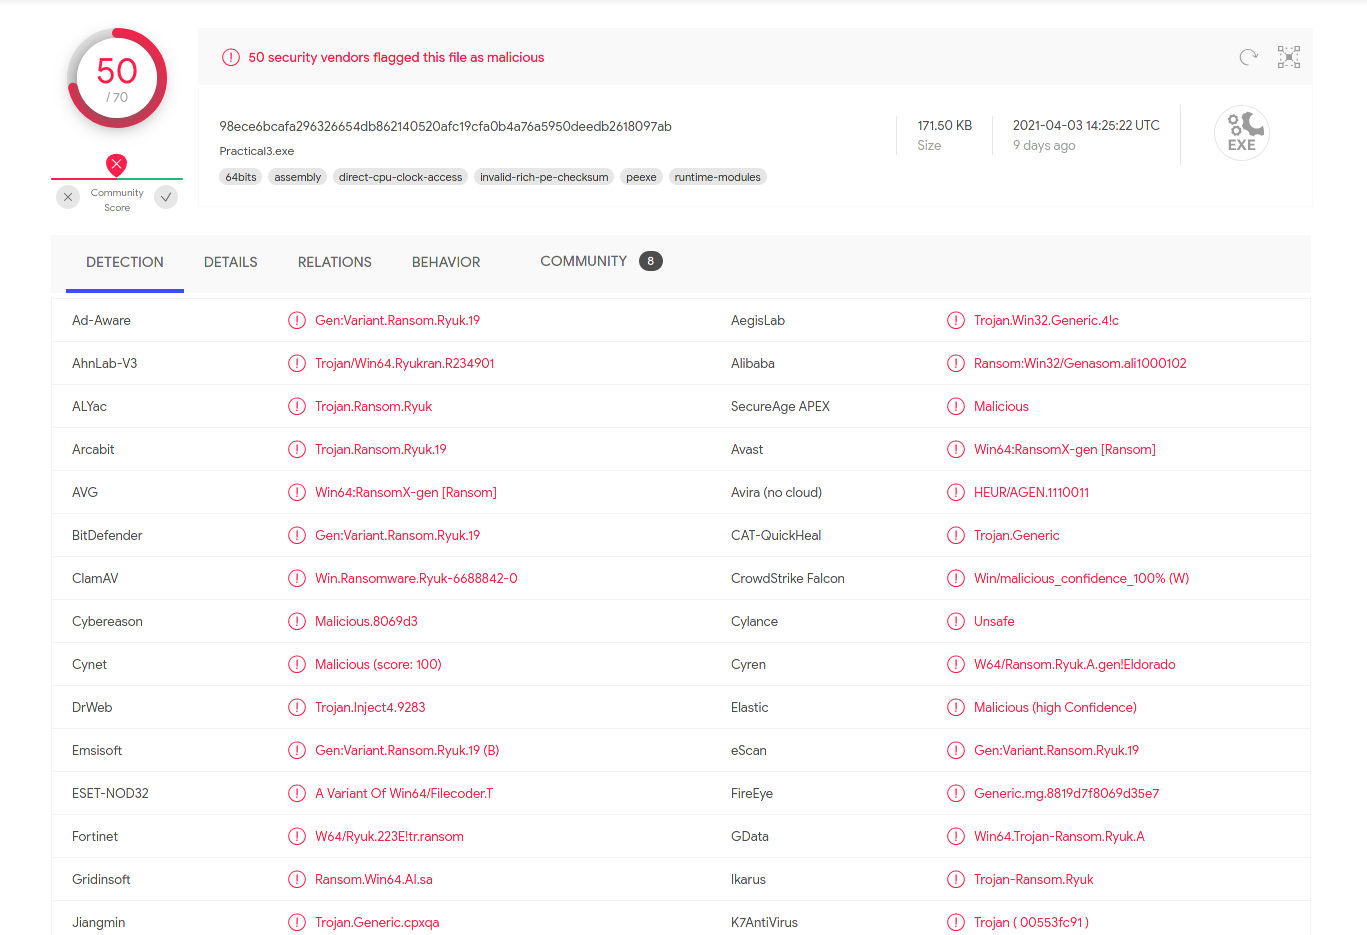
\includegraphics[width=\columnwidth]{pics/virustotal.png}
	\caption{VirusTotal: VirusTotal Scan}
	\label{virustotal}
\end{figure}

\begin{figure}[!htbp]% [!hb] forces image to be placed at that position
	\centering
	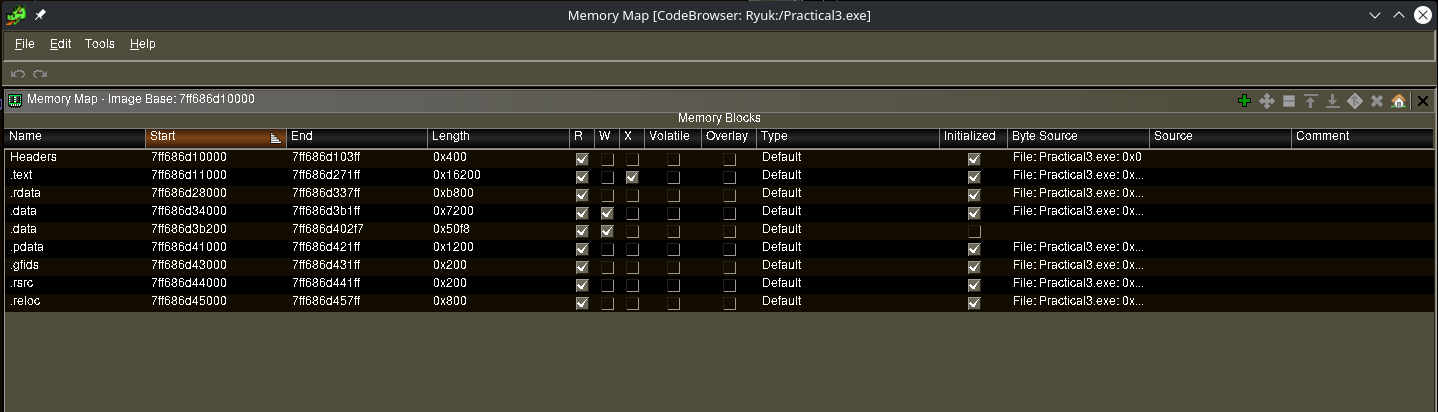
\includegraphics[width=\columnwidth]{pics/peHeaders.png}
	\caption{Ghidra: \textit{PE} headers}
	\label{peHeaders}
\end{figure}

\begin{figure}[!htbp]% [!hb] forces image to be placed at that position
	\centering
	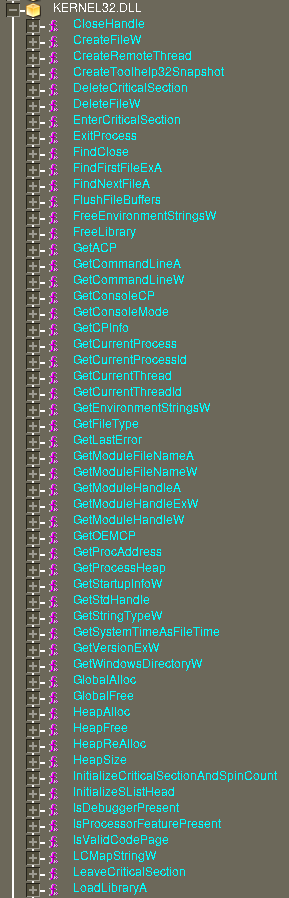
\includegraphics[width=\columnwidth]{pics/importsKernel32.png}
	\caption{Ghidra: \textit{Kernel32.dll} Imports}
	\label{importsKernel32}
\end{figure}

\begin{figure}[!htbp]% [!hb] forces image to be placed at that position
	\centering
	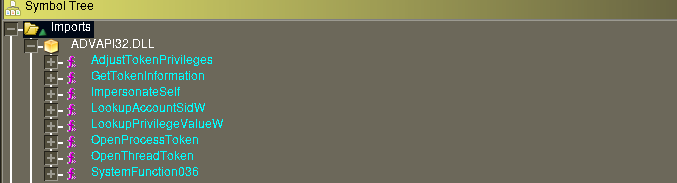
\includegraphics[width=\columnwidth]{pics/importsAdvapi32.png}
	\caption{Ghidra: \textit{Advapi32.dll} Imports}
	\label{importsAdvapi32}
\end{figure}

\begin{figure}[!htbp]% [!hb] forces image to be placed at that position
	\centering
	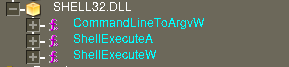
\includegraphics[width=\columnwidth]{pics/importsShell32.png}
	\caption{Ghidra: \textit{Shell32.dll} Imports}
	\label{importsShell32}
\end{figure}

\newpage
\printbibliography
\end{document}